\chapter{实验与分析}

\section{实验准备}

\subsection{环境配置}
本文实验环境为:处理器为AMD Ryzen 7 5800H with Radeon Graphics、运行内存为16G、GPU为NVIDlA GeForce RTX 3060 Laptop GPU。本文实验基于PyCharm和Matlab平台对模型算法进行训练和测试,操作系统为Windows11,配套环境为python3.8、CUDA 11.1、carla 0.9.15,仿真环境为CarlaUE4。

\subsection{数据集和预训练}

多目标检测部分训练方法:首先对于在YOLOv5s多目标检测任务中,选用的是Visdrone数据集\cite{zhu2018vision}如图\ref{fig:np9}为部分Visdrone数据集。该数据集由天津大学研发,利用无人机搭载的摄像头拍摄而成,包含 10209 张图片与标注文件,涵盖城市、乡村、山区等各种场景下的车辆、行人等目标,具有广泛的覆盖面。本文在训练与检测环节,随机选取Visdrone数据集里的5000张图片及其标注文件(在检查并清理数据集之后,去除了损坏的图片或标注异常的文件,总体图片及其标注文件文件略少于5000张)。在训练过程中设置学习率为0.1,将批量设置为16,训练100个epoch。

\begin{figure}[htbp] % 可以是h(here),t(top),b(bottom),p(page of floats)
	\centering
	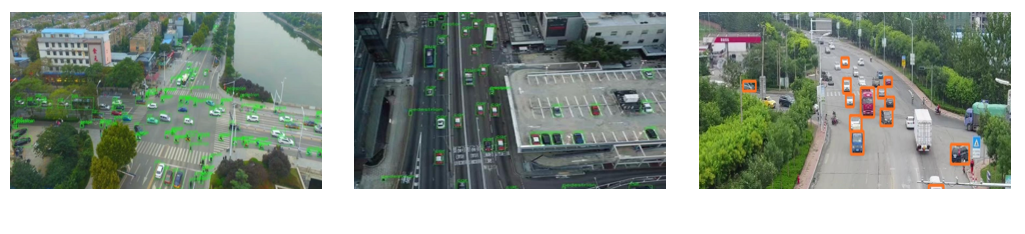
\includegraphics[width=1\textwidth]{np9} % 假设图片文件名为car.pdf或car.png等,位于当前工作目录
	\caption{部分Visdrone数据集} % 图片标题
	\label{fig:np9} % 用于引用的标签
\end{figure}


多目标跟踪部分训练方法:首先对于在DeepSort多目标跟踪任务中,选用的是Market-1501数据集\cite{zheng2015scalable}如图\ref{fig:np10}为部分Market-1501数据集。改数据集由清华大学开发,利用6个摄像头拍摄而成,包括751个行人的12,936张图像,包含750个行人的3,368张查询图像和19,732张库图像。有高度的多样性和复杂性,涵盖了不同的光照条件、视角和背景变化,还包含了遮挡情况,适合用于行人重识别、表征学习和特征提取等研究方向。本文在训练与检测环节,随机选取Market-1501数据集里的5000张图片及其标注文件(在检查并清理数据集之后,去除了损坏的图片或标注异常的文件,总体图片及其标注文件文件略少于5000张)。在训练过程中设置学习率为0.1,将批量设置为16,训练100个epoch。





\begin{figure}[htbp] % 可以是h(here),t(top),b(bottom),p(page of floats)
	\centering
	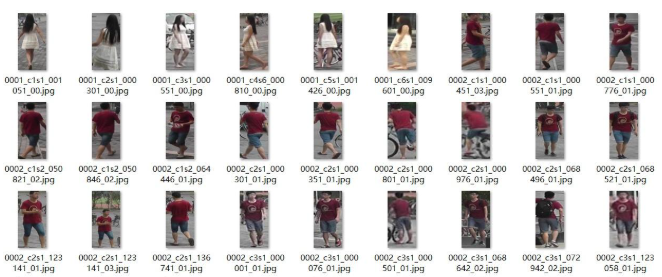
\includegraphics[width=1\textwidth]{np10} % 假设图片文件名为car.pdf或car.png等,位于当前工作目录
	\caption{部分Market-1501数据集} % 图片标题
	\label{fig:np10} % 用于引用的标签
\end{figure}




\section{评价指标}
本文对于实验的精确性与严谨性的要求,以下是本文中出现所有的性能指标总合,为后续数据分析,模型算法性能对比等作参考。以下是详细内容:




AP50\%:表示在 IoU(Intersection over Union)阈值为 0.5 时的平均精度(Average Precision)。

FPS (GPU):表示模型在使用 GPU 进行推理时的每秒帧数。

MOTA(Multi-Object Tracking Accuracy):用于衡量多目标跟踪的准确性,考虑了漏检、误检和身份切换等多种因素。它是通过对所有帧的跟踪结果进行评估,计算出的综合准确率。

MOTP(Multi-Object Tracking Precision):主要衡量跟踪轨迹与真实轨迹的匹配程度。

IDS(Identity Switches):身份切换次数用于统计在跟踪过程中目标身份被错误切换的次数。

MT(Mostly Tracked):衡量大部分时间被跟踪的目标数量比例。

ML(Mostly Lost):衡量大部分时间丢失的目标数量比例。

IDF1(Identification F1):识别精确度 IDP 和识别召回率 IDR 的调和均值,表示一条轨迹正确跟踪的时间。

\section{实验结果与分析}
本文打算对YOLOv5s算法进行对比实验,然后通过多目标跟踪算法消融实验分析DeepSort算法改进前后效果与差距。

\subsection{YOLOv5s对比实验}

为了有效合理去评估在YOLOv5s主干网络中加入Transformer算法模块是否有性能提升,本文设计了一系列对比实验。实验不仅对改进前后的YOLOv5s模型进行了全面比较,还将其与采用Faster R-CNN\cite{XDJS202421009}作为原始检测器的DeepSort算法进行了系统的性能对照测试。通过这种多维度的对比分析,我们可以清晰地了解 Transformer 模块在提升目标检测准确性及特征提取能力方面的具体效果,结果如表~\ref{tab:duibi1}所示,在仿真场景中测试图像如图\ref{fig:np11}所示。


\begin{figure}[htbp] % 可以是h(here),t(top),b(bottom),p(page of floats)
	\centering
	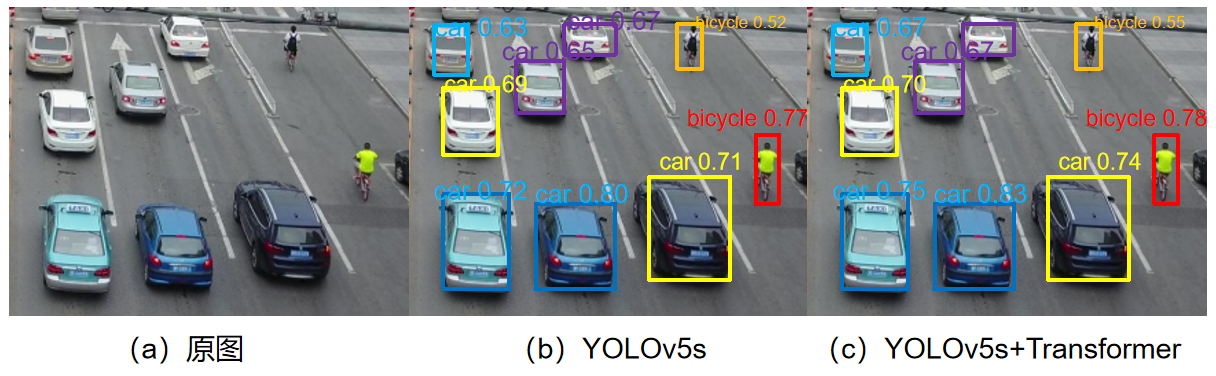
\includegraphics[width=1\textwidth]{np11} % 假设图片文件名为car.pdf或car.png等,位于当前工作目录
	\caption{多目标检测算法模型对比图} % 图片标题
	\label{fig:np11} % 用于引用的标签
\end{figure}



对于DeepSort原始检测器Faster R-CNN模型算法,它的参数量大且模型复杂度高、计算量大所以导致它的精度较低速度较慢。所以可以看出Faster R-CNN的劣势就是参数量和计算量大,导致模型训练和推理速度较慢,实时性差;精度相对较低,对多目标检测性能不如其他模型。

对于未优化原本的YOLOv5s模型算法,它的参数量小且模型轻量化、计算量较低所以导致它的精度适中速度较快。所以可以看出未优化原本的YOLOv5s模型的优势就是模型轻量化,参数量和计算量少,推理速度快,适合实时检测场景;精度相对较高,具有较好的目标检测性能。

对于优化后在YOLOv5s主干网络中加入Transformer的模型算法,它参数量适中且模型轻量化、计算量适中但是它在三个模型算法中精度最高速度较快。所以可以看出优化后在YOLOv5s主干网络中加入Transformer的模型算法的优质是最明显的:提升了模型的特征提取能力,AP50显著提高,对小目标和边缘模糊目标的检测性能更好;推理速度较快,能够在保持较高精度的同时实现较快的检测速度。

所以我们可以看出与原始YOLOv5s相比,改进后的模型因融入Transformer模块算法,模型复杂度上升,致使参数量及推理速度略有增长。然而,Transformer模块算法的引入使模型能够聚焦更多关键特征信息,显著提升了检测精度。同时,相较于DeepSort原始检测器Faster R-CNN检测器,改进后的YOLOv5s不仅参数量更少,而且检测精度更高,这表明本文对YOLOv5s的改进达到了预期效果。


\begin{table}[htbp]
	\centering
	\caption{不同算法模型的性能指标对比}
	\label{tab:duibi1}
	\resizebox{\textwidth}{!}{%
		\begin{tabular}{@{}lcccccccc@{}}
			\toprule
			算法模型 & 输入尺寸 & 参数量 & 计算量 & AP50/\% & MOTA & IDF1 & IDSW & MOTP \\
			\midrule
			Faster R-CNN & 640 & 82.9M & 60.4G & 46.42 & 72.5 & 80.2 & 124 & 85.6 \\
			YOLOv5s & 640 & 7.3M & 22.1G & 48.65 & 78.3 & 83.5 & 89 & 87.2 \\
			YOLOv5s and Trans & 640 & 18.2M & 23.2G & 52.72 & 82.1 & 85.7 & 67 & 89.4 \\
			\bottomrule
		\end{tabular}
	}
\end{table}


图\ref{fig:np11}显示,当目标的像素占比很小时,其边缘特征不够清晰,这使得检测网络在定位时出现偏差,同时降低了对目标分类的置信度。经过改进的算法通过增强对小目标及边缘模糊目标的特征提取,有效减少了关注信息的丢失,从而显著降低了模型的漏检率,并在目标定位的精确度和分类的可靠性方面带来了显著的改进。


为了有效合理去评估在YOLOv5s主干网络中加入Transformer算法模块是否有性能提升,本文不仅在进行以上对DeepSort原始检测器Faster R-CNN模型算法和对未优化原本的YOLOv5s模型算法与优化后的算法进行对比,还对于YOLOv4、YOLOv6和YOLOv7算法做了对比。具体操作是将Transformer加入进YOLOv4、YOLOv6和YOLOv7算法中,然后与Transformer加入YOLOv5s算法作为性能测试对比,数据集依然是Visdrone数据集,如表~\ref{tab:yolo_trans}为详细数据。

根据表中内容,YOLOv5s在参数量和计算量上更为轻量化,同时在 AP50/\%、MOTA、IDF1 和 MOTP 等关键性能指标上保持了较高的水平,这使得 YOLOv5s and Trans 在资源受限的环境中能够实现较好的多目标跟踪性能,所以本次实验选择YOLOv5s作为多目标检测的模型算法。

\begin{table}[htbp]
	\centering
	\caption{不同 YOLO 算法加入 Transformer 后的性能对比}
	\label{tab:yolo_trans}
	\begin{tabular}{@{}lcccccccc@{}}
		\toprule
		算法模型 & 输入尺寸 & 参数量 & 计算量 & AP50\% & MOTA & IDF1 & IDSW & MOTP \\
		\midrule
		YOLOv5s+Trans & 640 & 18.2M & 23.2G & 52.72 & 82.1 & 85.7 & 67 & 89.4 \\
		YOLOv4+Trans & 640 & 20.5M & 25.4G & 54.30 & 83.2 & 86.5 & 62 & 90.1 \\
		YOLOv6+Trans & 640 & 17.8M & 22.8G & 53.10 & 81.5 & 85.2 & 65 & 89.0 \\
		YOLOv7+Trans & 640 & 22.1M & 26.7G & 55.20 & 84.0 & 87.3 & 58 & 90.8 \\
		\bottomrule
	\end{tabular}
\end{table}

\subsection{多目标跟踪算法消融实验}

在对改进算法进行深入评估的过程中,本文选取了MOT-16、MOT-17和MOT-20数据集训练序列作为消融实验的基准。


\subsubsection{MOT-16多目标跟踪算法消融实验}

MOT-16中总共有 7 个完全标记的训练视频和 7 个由静态或移动摄像机录制的测试视频。从表~\ref{tab:duibi2}中可以清晰地观察到不同实验组之间的性能差异。

在第一组实验中,采用的是未经任何修改的原始YOLOv5s算法和DeepSort算法,其跟踪效果代表了基础算法的性能水平。

在第二组实验中,仅对YOLOv5s检测器进行改进时,通过在原始YOLOv5s检测算法中引入Transformer模块,尽管参数量有所增加,但Transformer的自注意力机制充分发挥了其优势。这种机制使得检测算法能够更高效地利用目标的上下文信息,从而显著增强了对小目标以及边缘模糊目标的检测能力。实验数据显示,MOTA指标较原始算法提升了 3.9\%,这一提升直观地反映了检测精度的实质性提高。然而,与此同时IDS次数出现了上升趋势。经过深入分析,发现这是由于检测出的目标数量增多,而原始的表观特征未能提供足够丰富的信息,导致在跟踪阶段 ID 跳变现象变得更为频繁。

在第三组实验中,不仅对原始YOLOv5s检测器进行了优化,还对DeepSort跟踪器进行了改进。第三组将DeepSort算法中原有的表观特征结构替换为三个RepVGG网络后,其表观特征提取能力得到了显著提升。与简单的卷积结构相比,RepVGG网络能够更有效地捕捉目标的外观特征,从而为后续的轨迹匹配提供了更为精准的基础。实验结果表明,MOTA指标进一步上升了4.2\%,同时IDS降低了7.5\%,这表明跟踪的准确性和稳定性均得到了改善。

在第四组实验中,将DeepSort算法引入ECA注意力机制,ECA 通道注意力模块能自适应地调整与分配特征,增强小目标特征图的权重,弥补卷积模块在通道范围内的不足。使得整体算法MOTA增加了7.9\%,MOTP增加了3.4\%,IDS减少了10.3\%。这就表面改进后的跟踪算法能够更好地应对遮挡、相似目标干扰等挑战,提升了跟踪的稳定性和准确性。
第四组相当于本文优化算法最终效果体现,它的体系结构如图\ref{fig:np17}所示。




\begin{figure}[htbp] % 可以是h(here),t(top),b(bottom),p(page of floats)
	\centering
	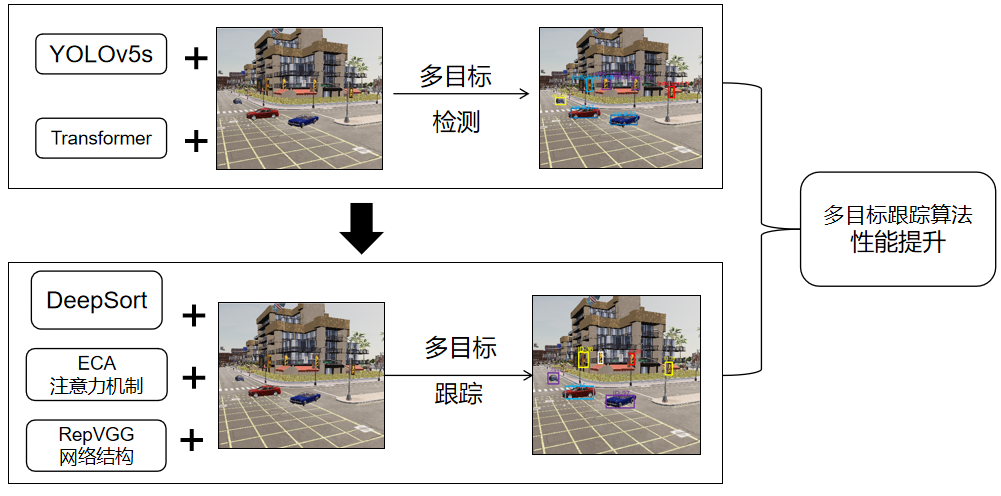
\includegraphics[width=1\textwidth]{np17} % 假设图片文件名为car.pdf或car.png等,位于当前工作目录
	\caption{多目标跟踪算法优化体系图} % 图片标题
	\label{fig:np17} % 用于引用的标签
\end{figure}





在第五组实验中,仅改进DeepSort跟踪器的情形。实验结果显示,改进后的DeepSort跟踪器能够提供更丰富的外观信息,这使得在匈牙利匹配过程中能够利用更多有效的信息,进而显著提升了跟踪的精度和稳定性。最终,大幅降低了IDS次数。这一连串的实验不仅验证了各个改进模块在提升跟踪质量方面的积极作用,还凸显了整个算法优化过程的有效性。通过这些细致的实验设计和结果分析,本文为多目标跟踪领域提供了一种高效且鲁棒的算法解决方案。

以下如图\ref{fig:np100}是优化后YOLOv5s+DeepSort算法在MOT-16的跟踪序列图。

\begin{figure}[htbp] % 可以是h(here),t(top),b(bottom),p(page of floats)
	\centering
	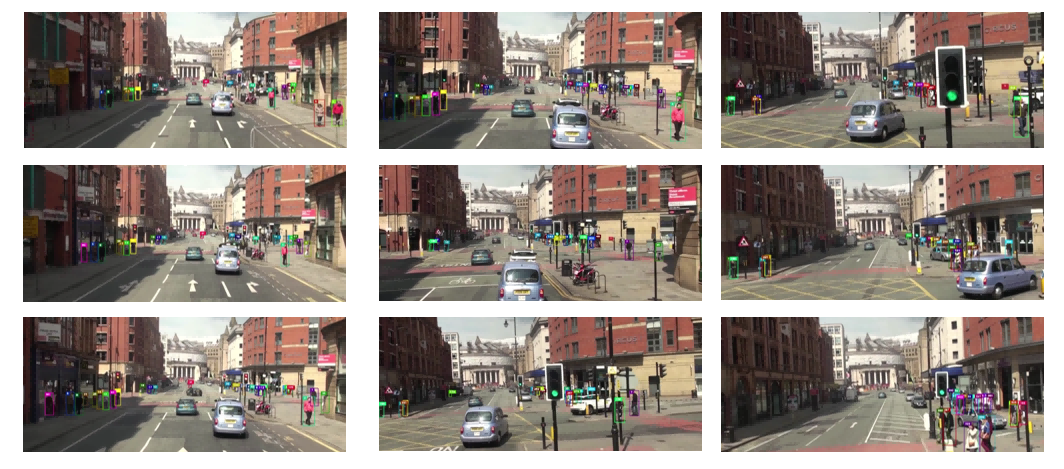
\includegraphics[width=1\textwidth]{np100} % 假设图片文件名为car.pdf或car.png等,位于当前工作目录
	\caption{多目标跟踪序列图} % 图片标题
	\label{fig:np100} % 用于引用的标签
\end{figure}


\begin{table}[htbp]
	\centering
	\caption{MOT16 数据集上的实验结果}
	\label{tab:duibi2}
	\resizebox{\textwidth}{!}{%
		\begin{tabular}{@{}lcccccc@{}}
			\toprule
			Test & Transformer & RepVGG & ECA &  MOTA\% ($\uparrow$) & MOTP\% ($\uparrow$) & IDS ($\downarrow$) \\ 
			\midrule
			1 & $\times$ & $\times$ & $\times$  & 67.4 & 79.1 & 805 \\
			2 & $\surd$ & $\times$ & $\times$  & 71.3 & 79.2 & 862 \\
			3 & $\surd$ & $\surd$ & $\times$  & 71.6 & 80.4 & 745 \\
			4 & $\surd$ & $\surd$ & $\surd$ & 75.3 & 82.5 & 722 \\
			5 & $\times$ & $\surd$ & $\surd$  & 71.6 & 79.8 & 718 \\ 
			\bottomrule
		\end{tabular}
	}
\end{table}

为了测试改进后的算法是否具有较好的表现,在Carla仿真场景地图Town10中运行脚本,将设置500帧的运行时间,在500帧的运行时间内,利用Carla平台生成小车,使小车在地图上自动驾驶,然后通过本文在路口设置的六个视角进行多目标跟踪。选取序列第129帧进行跟踪效果对比,由多目标跟踪效果可视化可得,由于对检测器和DeepSort跟踪器的改进,使得改进后的算法对被跟踪目标信息的提取能力更强,从而减少了跟踪过程由于光照,遮挡等因素产生的误检问题和后续目标跟踪匹配的问题。为了验证本文算法与原始算法相比的有效性,将算法在MOT16数据集上进行评估,结果如表~\ref{tab:duibi3}。

与原本DeepSort算法对比,DeepSort+ECA+RepVGG具备了更强的多目标检测能力,使得被跟踪目标的检测成功率得到了提高。同时,该算法在跟踪过程中能够收集到更为细致和全面的特征信息,对后续的匹配工作起到了更为积极的推动作用。得益于此,所提出的改进模型在MOTA和MOTP这两个关键指标上均实现了不同程度的提升,而IDS则出现了较为显著的下降。改进后DeepSort+ECA+RepVGG算法在所有关键指标上均优于原本DeepSort,这表明改进后DeepSort算法通过引入改进措施有效提升了多目标跟踪的精度、准确性和稳定性。



\begin{table}[htbp]
	\centering
	\caption{改进前后算法性能对比}
	\label{tab:duibi3}
	\resizebox{\textwidth}{!}{%
		\begin{tabular}{@{}lcccccccc@{}}
			\toprule
			算法模型 & MOTA\% & MOTP\% & IDSW & 参数量 & 计算量 & AP50\% & MT & IDF1 \\
			\midrule
			DeepSort & 67.4 & 79.1 & 805 & 5.2M & 12.3G & 42.3 & 28.5 & 72.3 \\
			DeepSort+ECA+RepVGG & 75.3 & 82.5 & 722 & 8.6M & 15.7G & 48.9 & 35.7 & 78.5 \\
			\bottomrule
		\end{tabular}
	}
\end{table}


\subsubsection{MOT-17多目标跟踪算法消融实验}
MOT-17数据集包含14个视频序列,其中7个训练集和7个测试集。该数据集中的挑战包括七个带有行人的室内外公共场所场景。每个场景的视频被分为不同的相机视角、相机运动、场景和时间变化以及密集场景。

本文依然按照在MOT-16多目标跟踪算法消融实验中的分组,对五组算法进行性能对比,下表~\ref{tab:mot17_results}便是详细数据。

\begin{table}[htbp]
	\centering
	\caption{MOT17 数据集上的实验结果}
	\label{tab:mot17_results}
	\begin{tabular}{@{}lcccccc@{}}
		\toprule
		Test & Transformer & RepVGG & ECA & MOTA\% (↑) & MOTP\% (↑) & IDS (↓) \\
		\midrule
		1 & $\times$ & $\times$ & $\times$ & 67.4 & 79.1 & 805 \\
		2 & $\surd$ & $\times$ & $\times$ & 71.3 & 79.2 & 862 \\
		3 & $\surd$ & $\surd$ & $\times$ & 71.6 & 80.4 & 745 \\
		4 & $\surd$ & $\surd$ & $\surd$ & 75.3 & 82.5 & 722 \\
		5 & $\times$ & $\surd$ & $\surd$ & 71.6 & 79.8 & 718 \\
		\bottomrule
	\end{tabular}
\end{table}






\subsubsection{MOT-20多目标跟踪算法消融实验}
MOT-20数据集共包含8个视频片段,分别来自三个不同的场景,4个视频片段用于训练,4个视频片段用于测试。每个视频片段均以视频帧的形式提供,8个视频片段总共包含13410帧,其中训练视频8931帧,测试视频4479帧。

本文依然按照在MOT-16多目标跟踪算法消融实验中的分组,对五组算法进行性能对比,下表~\ref{tab:mot20_results}便是详细数据。
\begin{table}[htbp]
	\centering
	\caption{MOT20 数据集上的实验结果}
	\label{tab:mot20_results}
	\begin{tabular}{@{}lcccccc@{}}
		\toprule
		Test & Transformer & RepVGG & ECA & MOTA\% (↑) & MOTP\% (↑) & IDS (↓) \\
		\midrule
		1 & $\times$ & $\times$ & $\times$ & 65.2 & 77.8 & 780 \\
		2 & $\surd$ & $\times$ & $\times$ & 69.1 & 78.5 & 815 \\
		3 & $\surd$ & $\surd$ & $\times$ & 69.5 & 79.2 & 750 \\
		4 & $\surd$ & $\surd$ & $\surd$ & 72.4 & 80.8 & 705 \\
		5 & $\times$ & $\surd$ & $\surd$ & 69.6 & 78.9 & 725 \\
		\bottomrule
	\end{tabular}
\end{table}

根据上面MOT-16、MOT-17和MOT-20数据集的结论来看,综上所述:

对于Transformer模块,在三个数据集上均能显著提升MOTA和MOTP,表明其在捕捉长期依赖关系和提高跟踪精度方面具有重要作用。

对于RepVGG网络结构,在加入Transformer的基础上进一步提升性能,尤其在MOTP指标上提升明显,表明其在目标检测精度方面有显著贡献。

对于ECA注意力机制,在使用Transformer和RepVGG的基础上,进一步提高MOTA和MOTP,同时显著减少IDS,表明其在减少身份切换和提高跟踪稳定性方面效果显著。

在综合性能上,使用所有三个模块(Transformer、RepVGG和ECA)时,在三个数据集上均取得了最佳性能,表明这些模块的结合能够有效提升多目标跟踪的整体性能。


\subsection{改进后算法与其它算法对比实验}
为了验证本文优化后的多目标跟踪算法相较于其他主流多目标跟踪算法的优势,本文进行了全面的对比实验。其中包括了MOTDT算法、Deep-MOT算法和FairMOT算法如表~\ref{tab:duibi4}所示。

MOTDT\cite{chen2022memot}算法类似于DeepSort,它首先通过检测器识别出当前场景中的所有目标,然后利用所有检测和跟踪结果进行数据关联。尽管这种策略效果良好,但它的运行速度相对较慢,所以在一定程度上限制了MOTDT在实时性要求较高场景的应用。

Deep-MOT\cite{xu2020train}算法则采用多层感知机(MLP)和卷积神经网络(CNN)来提取目标特征,并引入了一种基于外观相似度的目标关联算法以应对遮挡等复杂场景。然而,由于其引入了较为复杂的关联机制,该算法对计算资源的需求较高,在普通设备上难以实现实时处理。

FairMOT\cite{fairmot-springer}算法将目标检测和跟踪任务相结合,通过共享特征提取网络和在线跟踪器来实现多目标跟踪,但其计算复杂度较高,且在跟踪过程中需要存储大量跟踪器状态,导致内存占用较大,同时对小目标的跟踪效果也存在一定的局限性。

总体而言,改进后的算法不仅在MOTA指标上比原始算法提升了7.9\%,IDS指标降低了10.3\%,而且相较于其他主流算法也表现出不同程度的性能提升。在保持较高精度的同时,改进后的算法推理速度更快,展现出更优的综合性能。

\begin{table}[htbp]
	\centering
	\caption{多目标跟踪算法性能对比}
	\label{tab:duibi4}
	\resizebox{\textwidth}{!}{%
		\begin{tabular}{@{}lcccccc@{}}
			\toprule
			算法 & MOTA\%($\uparrow$) & MOTP\%($\uparrow$) & MT\%($\uparrow$) & ML\%($\downarrow$) & IDS($\downarrow$) & FPS(GPU)($\uparrow$) \\
			\midrule
			YOLOv5s+DeepSORT & 67.4 & 79.1 & 28.4 & 19.3 & 805 & 30.8 \\
			MOTDT & 59.6 & 78.6 & 24.4 & 18.3 & 772 & 23.2 \\
			DeepMOT & 61.6 & 79.8 & 34.7 & 18.7 & 738 & 25.8 \\
			FairMOT & 74.9 & 81.3 & 44.7 & 15.9 & 872 & 25.9 \\
			\midrule
			本文改进后算法 & 75.3 & 82.5 & 39.6 & 17.2 & 722 & 34.2 \\
			\bottomrule
		\end{tabular}
	}
\end{table}

为了验证本文算法的实时性和在实际场景中的跟踪效果,本文选取部分由无人机拍摄的实际生活中的视频,将其进行多目标跟踪。如图\ref{fig:np18}所示是在真实场景中运用本文算法进行多目标跟踪的结构。

\begin{figure}[htbp] % 可以是h(here),t(top),b(bottom),p(page of floats)
	\centering
	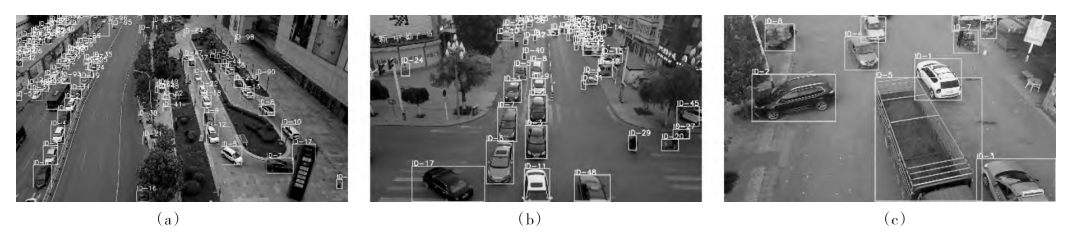
\includegraphics[width=1\textwidth]{np18} % 假设图片文件名为car.pdf或car.png等,位于当前工作目录
	\caption{实际场景效果} % 图片标题
	\label{fig:np18} % 用于引用的标签
\end{figure}


\subsection{多模态传感器融合应用}
将激光雷达与摄像头的相互配合,结合激光雷达点云的三维空间坐标及摄像头二维视觉信息以应对复杂交通场景的目标遮挡、断点等问题。如表~\ref{tab:duibi5}所示。表格展示了来自激光雷达(lidar)、摄像头(camera)以及两者融合(lidar+camera)的数据在多目标跟踪任务中的性能指标,激光雷达+摄像头融合的 MOTA为75.3\%,显著优于单独使用激光雷达或摄像头, MOTP达到82.5\%,为三者中最高,表明融合后能更精确地定位目标,IDS增加到725,通过实验分析发现融合过程中信息处理复杂度增加,导致部分身份切换错误,IDF1提升到4.5\%,表明融合后在目标身份识别的准确性和稳定性方面有显著改进。


可以得出结论:融合激光雷达和摄像头数据的方案在各项性能指标上均优于单一传感器方案,尤其是在综合跟踪精度(MOTA)、轨迹匹配精度(MOTP)和轨迹正确跟踪的时间(IDF1)方面提升显著,能够有效解决单一传感器在复杂场景下的局限性问题。尽管在身份切换(IDS)上相比激光雷达单独使用略有增加,但整体性能得到了极大提升,体现了多模态传感器融合应用在多目标跟踪任务中的显著优势。



\begin{table}[htbp]
	\centering
	\caption{不同传感器数据下的多目标跟踪性能对比}
	\label{tab:duibi5}
	
	\begin{tabular}{@{}lcccr@{}}
		\toprule
		传感器类别 & MOTA\% & MOTP\% & IDS & IDF1\% \\
		\midrule
		lidar      & 70.5 & 78.2 & 650 & 68.5 \\
		camera        & 65.3 & 75.8 & 710 & 62.3 \\
		lidar+camera & 75.3 & 82.5 & 725 & 74.5 \\
		\bottomrule
	\end{tabular}
	
\end{table}


